\chapter{Εισαγωγή}
\label{chapter:intro}

Ο όρος \emph{Τεχνητή Νοημοσύνη} αναφέρεται στην ικανότητα των υπολογιστικών
συστημάτων να μιμούνται στοιχεία της ανθρώπινης συμπεριφοράς.
Η επιθυμία των ανθρώπων να κατασκευάσουν "έξυπνες" μηχανές, καταγράφεται από
τα έτη της αρχαίας Ελλάδας. Μυθικές μορφές όπως οι Πυγμαλίωνας, Δαίδαλος και
Ήφαιστος μπορούν να θεωρηθούν ώς θρυλικοί εφευρέτες και δημιουργοί νοούντων
μηχανών όπως η Γαλάτεια, o Τάλος και η Πανδώρα.

Ένας πιο ολοκληρωμένος ορισμός της Τεχνητή Νοημοσύνη είναι:
\begin{displayquote}
\emph{
  Ο κλάδος/τομέας της επιστήμης της πληροφορικής, που ασχολείται
  με την σχεδίαση και κατακευή ευφυών συστημάτων, δηλαδή συστημάτων που
  κατέχουν χαρακτηριστικά που σχετίζονται με την ανθρώπινη νοημοσύνη και συμπεριφορά.
}
\end{displayquote}
Με την εμφάνιση των πρώτων ηλεκτρονικών και (επανα)προγραμματιζόμενων υπολογιστικών συστημάτων,
οι άνθρωποι ξεκίνησαν να σκέφτονται τρόπους για να κατασκευάσουν "έξυπνες" μηχανές.
H ραγδαία εξέλιξη στον κλάδο της επιστήμης της πληροφορικής, τις τελευταίες
δεκαετίες, έφερε και την εξέλιξη στην επιστήμη της Τεχνητής Νοημοσύνης.
Το 1997, η IBM κατασκεύασε ένα υπολογιστικό σύστημα το οποίο μπορούσε να
παίξει σκάκι (Deep Blue) \cite{campbell2002deep}, το οποίο κέρδισε τον παγκόσμιο
τότε πρωταθλητή στο σκάκι, Garry Kasparov. Το σκάκι έχει εξήντα τέσσερις θέσεις
και τριάντα δύο πιόνια που μπορούν να κινούνται με συγκεκριμένο τρόπο. H μηχανή
Deep Blue, μπορούσε να εκτιμήσει και να αξιολογήσει διακόσια εκατομμύρια
πιθανές καταστάσεις της σκακιέρας. Ωστόσο, πρέπει να σημειώσουμε ότι η επίλυση του
προβλήματος του σκακιού, είναι ένα απλό πρόβλημα το οποίο μπορεί να περιγραφεί
πλήρως μέσα από μια λίστα με κανόνες.
%\begin{figure}[!ht]
  %\centering
  %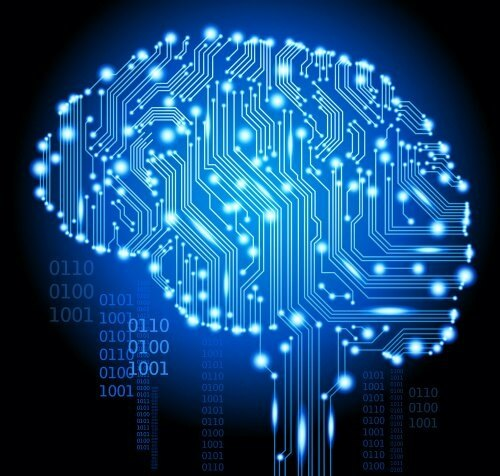
\includegraphics[width=0.7\textwidth]{./images/chapter3/building_a_brain.jpg}
  %% \caption[Τεχνητή Νοημοσύνη]{Τεχνητή Νοημοσύνη}
  %\label{fig:AI_1}
%\end{figure}
Η δυνατότητα ενός "ευφυούς" ρομποτικού συστήματος να αντιλαμβάνεται
το περιβάλλον του, είναι απαραίτητη ικανότητα που πρέπει να διαθέτει.
Ένας ρομποτικός πράκτορας, σε πληθώρα εφαρμογών, πρέπει να διαθέτει τόσο την
ικανότητα να αναγνωρίζει, μέσω εικόνων λήψης από κάμερας, διάφορα αντικείμενα,
όσο και την ικανότητα να εντοπίζει επακριβώς την θέση του
εκάστοτε αντικειμένου στον χώρο. Δεν θα είχε νόημα για ένα ρομπότ, να έχει άποψη
για την παρουσία αντικειμένων γύρω του, αν δεν έχει και την ικανότητα να γνωρίζει
και την θέση των αντικειμένων αυτών.

Σήμερα, το γενικότερο πρόβλημα της αναγνώρισης και εντοπισμού αντικειμένων σε εικόνες
λύνεται με την χρησιμοποίηση Νευρωνικών Δικτύων Συνέλιξης (Convolutional Neural Networks - CNN).
Το γεγονός ότι τα CNN έχουν την δυνατότητα να κατηγοριοποιήσουν αντικείμενα,
σε προβλήματα όπου οι κλάσεις αντικειμένων κυμένονται από δεκάδες έως και χιλιάδες,
θέτει το ερώτημα της εφαρμογής τους σε εφαρμογές πραγματικού χρόνου εφαρμογές
με ιδιαίτερο ενδιαφέρον στην επιστήμη της ρομποτικής.
\\

\textbf{TODO: More...!!!???}

\section{Περιγραφή του Προβλήματος}
\label{section:problem_description}

Ο μεγάλος χρόνος που χρειάζεται ένα CNN, τόσο για να κατηγοριοποιήσει, όσο και
για να εντοπίσει, ένα αντικείμενο το κάνει ακατάλληλο για χρήση σε εφαρμογές πραγματικού
χρόνου. Αυτό συμβαίνει λόγω του "βάθους" που έχουνε τα νευρωνικά αυτά δίκτυα.
Είναι ιδιαίτερα σηματνικό, ένα ρομπότ να μπορεί να αντιλαμβάνεται το περιβάλλον
του; να μπορεί να αναγνωρίζει ανθρώπους, ζώα, αντικείμενα γενικότερα. Ωστόσο,
θέλουμε τα ρομπότ να είναι και όσο πιο "ελκιστικά" γίνεται στον άνθρωπο ή/και μικρότερα.
Αυτό, φέρει σαν αποτέλεσμα να μην μπορούμε να φορέσουμε μεγάλα, με μεγάλη,
υπολογιστική ισχύ, υπολογιστικά συστήματα, κατευθείαν πάνω στα ρομπότ.


\section{Σκοπός - Συνεισφορά της Διπλωματικής Εργασίας}
\label{section:contribution}

H συγκεκριμένη διπλωματική εργασία
καταπιάνεται με τα πρόβλημα της αναγνώρισης αντικειμένων σε VGA frames (640 x 480)
σε πραγματικό χρόνο, χρησιμοποιώντας Νευρωνικά Δίκτυα Συνέλιξης (CNN).
Περαιτέρω, στοχεύει στην ανάπτυξη και εφαρμογή των νευρωνικών αυτών δικτύων
σε ρομποτικά συστήματα όπου η επεξεργαστική ισχύ είναι χαμηλή, σε σύγκριση με
σταθερά υπολογιστικά συστήματα.
...



\section{Διάρθρωση της Αναφοράς}
\label{section:layout}

DOCUMENT SECTION here!

Η διάρθρωση της παρούσας διπλωματικής εργασίας είναι η εξής:

\begin{itemize}
  \item {Στο \textbf{Μέρος Ι} περιγράφονται ορισμένες εισαγωγικές έννοιες και
      βασικές γνώσεις, ώστε ο αναγνώστης να κατανοήσει με μεγαλύτερη ευκολία
      τα αντικείμενα που πραγματεύεται η διπλωματική εργασία.
      Ειδικότερα, τα κεφάλαια είναι:
      \begin{itemize}
        \item{\textbf{Κεφάλαιο 2:} Παρατίθεται η ανασκόπηση της ερευνητικής
            περιοχής αναφορικά με τα αντικείμενα στα οποία επιδιώκει να
            παρουσιάσει λύσεις η διπλωματική εργασία.
          }
        \item{\textbf{Κεφάλαιο 3:} Περιγράφονται τα βασικά θεωρητικά στοιχεία
            στα οποία βασίστηκε η παρούσα υλοποίηση, καθώς επίσης και οι
            διάφορες τεχνικές και τα εργαλεία που χρησιμοποιήθηκαν.
          }
      \end{itemize}
    }
  \item{Το \textbf{Μέρος ΙΙ} αποτελείται από τρία κεφάλαια στα οποία
      περιγράφονται πλήρως η υλοποιήσεις.
      %\begin{itemize}
      %\end{itemize}
    }
  \item{Στο \textbf{Μέρος ΙΙΙ} παρουσιάζεται αναλυτικά η μεθοδολογία των
      πειραμάτων, τα αποτελέσματά τους και τα συμπεράσματα στα οποία καταλήξαμε.
      Τέλος, γίνεται αναφορά σε διαδικαστικά προβλήματα που ανέκυψαν
      και προτείνονται θέματα για μελλοντική μελέτη.
      %\begin{itemize}
      %\end{itemize}
    }
\end{itemize}




